%-------------------------------- Configurações --------------------------------

\documentclass[a4paper,         % Tamanho do papel: A4
	           abntfigtabnum,
	           noindentfirst,
	           normaltoc,
	           pnumplain,
	           notimes
	           % capchap,
]{abnt}

% Links border color
\newcommand{\bc}{NavyBlue}

\usepackage[utf8]{inputenc} % para pode escrever caracteres acentuados normalmente
\usepackage[brazil]{babel}
\usepackage{graphicx}
\usepackage[usenames,dvipsnames]{xcolor} % http://en.wikibooks.org/wiki/LaTeX/Colors
\usepackage[pdfborder={0 0 0},pdfborderstyle={/S/U/W 0.5},citebordercolor=\bc,filebordercolor=\bc,urlbordercolor=\bc,linkbordercolor=\bc]{hyperref} % http://www.tug.org/applications/hyperref/manual.html e http://migre.me/7FH3e
\usepackage[alf]{abntcite}
\usepackage{booktabs} % para utilização das linhas separadoras na tabela
\usepackage{listings} % http://linorg.usp.br/CTAN/macros/latex/contrib/listings/listings.pdf
\usepackage{textcomp}
\usepackage{minted} % foi adicionado o seguinte hack no minted: http://migre.me/7M8wI

%--------------------------- Minted Highligthing -------------------------------

\renewcommand\listingscaption{Código}

% http://github.com/hugomaiavieira/pygments-style-github
\usemintedstyle{github}

% O minted é tipo uma extensão do fancyvrb. Então, algumas modificações nele
% são feitas de acordo com o fancyvrb.
% Documentação do fancyvrb: http://linorg.usp.br/CTAN/macros/latex/contrib/fancyvrb/fancyvrb.pdf

% Ajustar o estilo do número, de acordo com o fancyvrb.
\renewcommand{\theFancyVerbLine}{\textcolor{Gray}{\scriptsize\arabic{FancyVerbLine}}}

% Ajusta estilo do caption. http://linorg.usp.br/CTAN/macros/latex/contrib/caption/caption-eng.pdf
\usepackage{caption}
\DeclareCaptionStyle{code_style}{margin=2mm}
\DeclareCaptionFont{code_font}{\footnotesize\bfseries}
\captionsetup[listing]{style=code_style,labelfont=code_font,textfont=code_font}

% Criando um novo comando para facilitar a adição de códigos
% http://tex.stackexchange.com/questions/42393/new-environment-with-minted
\makeatletter
\newenvironment{mycode}[3]
 {\VerbatimEnvironment
  \minted@resetoptions
  \setkeys{minted@opt}{linenos,fontfamily=courier, fontsize=\scriptsize, xleftmargin=21pt}
  \renewcommand{\minted@proglang}[1]{#1}
  \begin{listing}[h]
    \caption{#2}\label{#3}
      \begin{VerbatimOut}{\jobname.pyg}}
 {\end{VerbatimOut}
  \minted@pygmentize{\minted@proglang{}}
  \DeleteFile{\jobname.pyg}
  \end{listing}}
\makeatother

%--------------------------------- Informações ---------------------------------

% http://www.tug.org/applications/hyperref/manual.html
\hypersetup{
  pdftitle=Técnicas emergentes de desenvolvimento de software,
  pdfauthor=Hugo Henriques Maia Vieira
  % pdfsubject={},
}

\begin{document}

\titulo{Técnicas emergentes de desenvolvimento de software}
\autor{Hugo Henriques Maia Vieira}
\instituicao{Universidade Estadual do Norte Fluminense Darcy Ribeiro}
\orientador{Rodrigo Soares Manhães, M.Sc.}
\comentario{Monografia apresentada ao Curso de Graduação em Ciência da
Computação da Universidade Estadual do Norte Fluminense Darcy Ribeiro como
requisito para obtenção do título de Bacharel em Ciência da Computação, sob
orientação do Prof. Rodrigo Soares Manhães, M.Sc.}
\local{Campos dos Goytacazes/RJ}
\data{2012}


\capa
\folhaderosto

\begin{titlepage}
 \vspace*{5cm}
 \begin{flushright}
  ``Ao infinito... e além!''\\\textit{Buzz Lightyear}
  \vspace{1cm}
 \end{flushright}

 \begin{flushright}
  ``As pessoas boas devem amar seus inimigos''\\\textit{Seu Madruga}
  \vspace{1cm}
 \end{flushright}
\end{titlepage}

\begin{center}
\textbf{AGRADECIMENTOS} \\ [2.5cm]
\end{center}

À meu pai Roosevelt, meu melhor amigo e grande companheiro, por estar sempre presente em todos os momentos felizes e tristes da minha vida e por ser a pessoa mais importante na formação do meu caráter, por eu me tornar quem sou.

À minha mãe e minhas irmãs, que mesmo distantes estão sempre por perto.

À minha namorada Alice, pelo amor, companheirismo e paciência.

Ao amigo e professor Rodrigo, por me mostrar o caminho da luz e por ser meu grande mestre e orientador.

À professora Sahudy, por ter sido parte fundamental da minha formação, acadêmica, profissional e pessoal.

À professora Annabell, por todo companheirismo e carinho, por mostrar que o trabalho duro é recompensador.

Ao professor Rivera por sua dedicação ao buscar sempre um curso melhor.

Ao professor Rogério, representando o NSI, por ter me aberto as portas para a área que adoro e escolhi seguir em minha vida profissional.

À todos meu amigos de curso, especialmente meus também companheiros de Algorich, Eduardo, Herond e Rafael por estarem presentes nos momentos mais dramáticos e nos mais engraçados.

À toda minha família, meus avós, meus primos e meus tios, por todo o suporte e felicidade que me proporcionam sempre.

\listoffigures

\begin{resumo}
Aqui entra o resumo do meu trabalho que será a última coisa a ser feita.
\end{resumo}

\sumario

\chapter{Introdução}

Com o passar dos anos, principalmente em uma época onde a tecnologia e os negócios mudam e evoluem de modo extremamente rápido, o mercado demanda e espera software inovadores e de alta qualidade, que sejam adequados a suas necessidades $-$ e o mais rápido possível \cite{TheBusinessOfInnovation}.

O desenvolvimento ágil de software, que neste ano de 2012 completa 11 anos, foi elaborado \cite{AgileManifesto} visando atender à estas expectativas do mercado, focando o processo de desenvolvimento nas pessoas e abraçando as mudanças que  naturalmente surgem durante a construção do software. De acordo com \citeonline{PMNetworkFailureDrop}, o \textit{Chaos Manifesto 2011}\footnote{O \textit{Chaos Manifesto} é uma pesquisa bienal realizada pelo \textit{The Standish Group} e teve início em 1994. As pesquisas publicadas em um ano representam os dados do ano anterior.} mostra que os resultados de 2010 representam, desde sua primeira edição, a maior taxa de sucesso nos projetos de desenvolvimento de software, que aumentou de 32\% em 2008 para 37\% em 2010. Segundo \citeonline{ResumoChaosReport}, o \textit{The Standish Group} conclui que uma das razões para o aumento da taxa de sucesso foi a utilização das metodologias ágeis, que cresce a uma taxa de 22\% CAGR\footnote{\href{http://en.wikipedia.org/wiki/Compound_annual_growth_rate} {Compound annual growth rate}} e hoje são adotados em 9\% de todos os projetos de Tecnologia da Informação em andamento e em 29\% dos novos projetos.

Como a adoção do desenvolvimento ágil é crescente nos últimos anos, diversos métodos e técnicas vem sendo desenvolvidos tendo como base os princípios e valores ágeis \cite{BDDRodrigo}, principalmente relacionadas ao teste de software e que serão abordadas no presente trabalho, sendo elas o Desenvolvimento Guiado por Testes (do inglês, \textit{Test-Driven Development} - TDD)\nomenclature{TDD}{Test-Driven Development}, Desenvolvimento Guiado por Comportamento (do inglês, \textit{Behaviour-Driven Development - BDD})\nomenclature{BDD}{Behaviour-Driven Development}, Integração Contínua e Dublês de Teste. Sendo técnicas emergentes, ainda são pouco discutidas no meio acadêmico, este trabalho pretende contribuir com esta discussão e com a introdução destas técnicas emergentes na academia.


\section{Justificativas e objetivos}

Existem poucos trabalhos acadêmicos no que se refere a técnicas emergentes de testes de software, como notado também por \citeonline{BDDSolis}, que em 2011 foram os primeiros a ter um artigo publicado sobre Desenvolvimento Guiado por Comportamento (BDD), pela \textit{IEEE Computer Society}.

Sendo assim, o objetivo do presente trabalho é contribuir com a introdução de técnicas e discussões surgidas no meio empresarial para a academia, além de agregar conhecimentos, ora dispersos e difusos, sobre as diferentes abordagens, possibilidades e pontos em aberto no emprego de tais técnicas.

As técnicas que serão abordadas neste trabalho tem seu conceito definido no mercado e evoluem através da evolução das ferramentas que os implementam. O fluxo de evolução é o seguinte:

\begin{figure}[h]
  \center
  \caption{Fluxo de evolução dos conceitos e ferramentas}
  \includegraphics[scale=0.60]{images/fluxo-conceito-ferramenta}
  \label{img:fluxo_conceito_ferramenta}
\end{figure}

Primeiramente cria-se um conceito e, em seguida, uma ferramenta que o implemente. Com base na utilização e observação desta ferramenta, há uma percepção de novas necessidades, fazendo que os conceitos evoluam e novas ferramentas sejam criadas.

Desta forma, a evolução das ferramentas e a evolução conceitual estão intimamente ligadas. No texto original sobre BDD \cite{IntroducingBDD} já se encontra isto. A inspiração para a criação de BDD foi uma ferramenta chamada \textit{AgileDox}\footnote{Mais informações em \url{http://agiledox.sourceforge.net}}, que fez o autor antever as novas possibilidades que cristalizou no conceito de BDD. Justamente por esta característica dinâmica, a informação e os diferentes conceitos estão dispersos, pois nunca foram sistematizados, ficando em uma espécie de ``inteligência coletiva"\ da comunidade de desenvolvimento ágil.

Além disso, como o presente trabalho está no contexto dos métodos ágeis, e nestes as partes conceitual e prática formam um todo inseparável, para toda técnica abordada serão utilizados exemplos mostrando código de um projeto real.

\section{Metodologia}

Será feita uma explanação sobre cada técnica e uma discussão comparando as diferentes abordagens, possibilidades e pontos em aberto no emprego de cada técnica.

Como base para a discussão, será utilizado o kanban-roots\footnote{\url{http://github.com/hugomaiavieira/kanban-roots}}, que foi desenvolvido pelo autor do presente trabalho utilizando todas as técnicas abordadas neste, possibilitando desta forma a obtenção de dados e experiências da utilização das técnicas em um projeto real.

O kanban-roots é um kanban\footnote{O termo tem origem no sistema Toyota de produção, onde kanban é a maneira como é coordenado o fluxo de peças na cadeia de suprimentos  \cite{AMaquinaQueMudouOMundo}. No contexto do presente trabalho, kanban é um quadro para visualização do fluxo de trabalho (tarefas) em um projeto.} online para auxiliar a organização e acompanhamento das tarefas em um projeto, sendo especialmente interessante para projetos \textit{opensouce} ou, de modo geral, para projetos com equipes geograficamente distribuídas.

Na figura \ref{img:tela_kaban_roots} pode ser visto um \textit{screen shot} do kanban de um projeto no kanban-roots.

O kanban é muito utilizado em metodologias ágeis como XP e Scrum como um quadro para visualização do fluxo de tarefas nas iterações de um projeto (mais na Seção \ref{sub:agilismo}). As tarefas inicialmente são posicionadas na divisão \textbf{\textit{Backlog}} até serem escolhidas para fazer parte de uma iteração. Nesse momento, as tarefas escolhidas vão para a divisão \textbf{\textit{To Do}} até que sejam escolhidas por um desenvolvedor para serem implementadas, passando para a divisão \textbf{\textit{Doing}}. Após o desenvolvedor concluir a tarefa, esta vai para a divisão \textbf{\textit{Done}}. Dessa maneira, todos os participantes tem a possibilidade de ver como está o andamento da iteração, além de ser possível acompanhar o que cada integrante do projeto está está fazendo naquele instante.

O kanban-roots já está em produção e vem sendo testado e utilizado com sucesso por algumas pessoas em empresas do Brasil como a Algorich, Voxline, Mandic, Quatix, mas também estrangeiras como a infoPiiaf e Free.fr (França), Ginzametrics (Estados Unidos), Osube (China), Centah (Canadá), Podmoskovie.info (Rússia), EvoEnergy (Inglaterra), Forgotten Labs (Lituânia), entre outros.

\begin{figure}[h]
  \center
  \caption{Tela do kanban de um projeto no kanban-roots}
  \includegraphics[scale=0.45]{images/kanban-roots}
  \label{img:tela_kaban_roots}
\end{figure}

Todos os trechos de código apresentados neste trabalho são trechos retirados do kanban-roots e a primeira linha de cada trecho sempre será um comentário informando o nome do arquivo original em que o dado trecho se encontra.

\section{Ferramentas utilizadas}

Para o desenvolvimento do kanban-roots foram utilizadas diversas ferramentas, sendo importante citar em que contexto e momento cada uma delas é utilizada.

Como base para o desenvolvimento, foi utilizado o \textit{framework web} Ruby On Rails\footnote{\url{http://rubyonrails.org}}. Para os testes de unidade apresentados na Seção \ref{sub:tdd} foi utilizado o Test::Unit\footnote{\url{http://test-unit.rubyforge.org/}}. Já na Seção \ref{sub:bdd} é utilizado o Rspec\footnote{\url{http://rspec.info/}} para testes unitários, testes de aceitação e dublês de teste. Ainda na Seção \ref{sub:bdd} também foi utilizado o Cucumber\footnote{\url{http://cukes.info/}} para testes de aceitação. Além dessas ferramentas, também foi utilizado o FactoryGirl\footnote{\url{https://github.com/thoughtbot/factory_girl}} para \textit{fixtures replacement} em todos os momentos em que se fez necessário.

\section{Trabalhos relacionados} % (fold)
\label{sec:trabalhos_relacionados}

\textbf{TODO: puxar os trabalhos relacionados de todas as técnicas abordadas}

Não existem muitos trabalhos acadêmicos relacionados às técnicas abordadas no presente trabalho, e todos eles abordam o tema apenas conceitualmente, deixando uma lacuna em termos de contextualização.

\citeonline{BDDSolis} apresentam algumas das principais características do \textit{Behaviour-Driven Development} (BDD), tendo como base uma pequena quantidade de estudo publicados sobre o tema e as ferramentas existentes para a utilização da técnica.

Sobre \textit{Test-Driven Development} (TDD), praticamente são apenas encontrados estudos empíricos, com estudos de caso na academia e na indústria, que discutem a efetividade do uso do TDD. Na Seção \ref{sub:a_efetividade_do_tdd} será feita uma análise destes estudos.

% section trabalhos_relacionados (end)
\chapter{Fundamentação teórica}

\section{Agilismo}

Em 2001 um grupo de dezessete especialistas, reconhecidos pela comunidade como
grandes nomes do desenvolvimento software, se reuniram para discutir sobre um
crescente conjunto de métodos que vinham surgindo e decidiram usar o termo
Agilismo para descrever essa nova geração de métodos ágeis \cite{AgileStory}.
Eles também escreveram o Manifesto Ágil \cite{AgileManifesto}, delineando um
conjunto de valores e princípios que, em resumo, trilham um
caminho para a eliminação de documentação e processos desnecessários, buscando
a simplicidade, com foco na geração de valor e proximidade com o cliente, além
de possibilitar respostas rápidas e eficazes às mudanças.

Pode-se dizer então, que o Desenvolvendo Ágil, ou Agilismo, é um rótulo genérico
para os métodos de desenvolvimento de software baseados no Manifesto Ágil
\cite{BDDRodrigo}.


\section{Técnicas}

\subsection{Test-Driven Development}
``Apenas escrever código para corrigir um teste falhando". Segundo
\citeonline{TestDrivenKoskela}, isto é \textit{Test-Driven Development} (TDD)
\cite{TDDbyExample} em apenas uma sentença.

O TDD é uma técnica onde o desenvolvimento do software é guiado por testes
automatizados, que são escritos antes de qualquer linha de código. Primeiro
escreve-se um teste, depois escreve-se o código para passar neste teste. Em
seguida, o código é refatorado para encontrar um design melhor, contanto sempre
com os testes existentes para que não sejam introduzidas falhas em outras partes
do sistema.

Esta abordagem encoraja bom design, produz código testável e mantém longe a
sobre-engenharia por conta de falsas suposições, pois, nos testes, é
especificado o que é desejado e escreve-se o código para fazer apenas aquilo que
realmente é necessário. \cite{TestDrivenKoskela, TDDbyExample, EmpiricalTDD}

Mas TDD é uma técnica emergente? Não e sim.

O TDD vem sendo utilizado esporadicamente há anos, contudo, não existia um nome
para identificar essa forma de desenvolver software. No entanto, em termos de
adoção, TDD continua sendo novo. \cite{TestDrivenKoskela, TDDbyExample, EmpiricalTDD}
Hoje, esta técnica tem um nome e começa a ganhar força, sendo utilizada em times
de grandes empresas como Google, Yahoo, Microsoft e IBM. \cite{EmpiricalTDD}



\subsection{Behaviour-Driven Development}

Criado em 2006 \cite{IntroducingBDD}, Behaviour-Driven Development (BDD) é uma
técnica de desenvolvimento de software cuja amplitude se estende às atividades
de design, documentação, validação e verificação, tratando-as de modo unificado
\cite{BDDRodrigo}.

O BDD é uma evolução do TDD. A grande diferença entre os dois, é que TDD não
abrange a validação do software, ou seja, se o software atende os requisitos.
Isso muda tudo, pois em BDD, o pensamento não é voltado à verificação, mas sim
no comportamento, em \textbf{validar} que o software faz o que deveria fazer,
sem deixar também de \textbf{verificar} se está funcionando como deveria.

BDD vem se tornando um consenso em automação de testes. Contudo, existe
controvérsia sobre seu modo de utilização.





\subsection{Integração contínua}

Em uma equipe com vários desenvolvedores, todos trabalhando na elaboração de um
mesmo sistema, existe o problema de unificar as diversas alterações feitas na
base de código, assegurando que a base continua consistente \cite{ImproveitCI}.
Para resolver esse problema, entra em cena a Integração Contínua (IC), que além
disso, tem como ponto chave dar um feedback rápido quando a base não está
consistente.

\cite{FowlerCI} definiu a IC da seguinte maneira:

\begin{citacao}
Integração Contínua é uma prática de desenvolvimento de software onde os membros
de um time integram seu trabalho frequentemente, geralmente cada pessoa integra
ao menos uma vez ao dia - podendo haver múltiplas integrações por dia. Cada
integração é verificada por um \textit{build} automatizado (incluindo testes)
para detectar erros de integração o mais rápido possível. Muitos times acham que
essa abordagem leva a uma significante redução nos problemas de integração e
permite que um time desenvolva software coeso mais rapidamente.
\end{citacao}

A IC é um dos pilares da agilidade, pois garante que todo o sistema funcione de
forma coesa a cada \textit{build}, mesmo que sua equipe seja grande e diversas
partes do código estejam sendo alteradas ao mesmo tempo \cite{CaelumCI}.

Existe um debate sobre a periodicidade da integração, que tem relação direta com
o tempo de execução da \textit{build}. Para assegurar o rápido feedback, esse
tempo de execução deve ser o menor possível, tentando manter sempre menor do que
dez minutos \cite{FowlerCI}.



\subsection{Dublês de Teste}

Em algumas ocasiões é difícil testar alguns componentes porque eles dependem de
outros componentes que não podem ser utilizados em ambiente de teste. Estas
situações podem acontecer por esses componentes não estarem disponíveis, por
eles não retornam os resultados necessários ou porque executá-los iria trazer
efeitos colaterais indesejados. Em outros casos, nossa estratégia de testes
requer que nós tenhamos mais controle do comportamento interno do componente.

Quando estamos escrevendo um teste onde não podemos/escolhemos usar componentes
reais, podemos substitui-los pelos Dublês de Teste que oferecem uma maneira de
isolar as dependências ao criar seus testes, permitindo a utilização de
componentes falsos para cumprir os papéis de componentes reais. Com isso,
eliminamos complexidade do código dos testes, pois mantemos o código de
implementação dos objetos pequeno e com baixo acoplamento.

Os Dublês de Teste não precisam se comportar exatamente como o componente real,
eles devem apenas prover a mesma API que o componente real.

\citeonline{XUnit} Define cinco categorias de Dublês de Teste:

\begin{itemize}
    \item
        Objetos \textbf{\textit{Dummy}} geralmente são utilizados apenas para
        preencher uma lista de parâmetros e nunca são realmente usados.

    \item
        Objetos \textbf{\textit{Fake}} são utilizados para substituir
        funcionalidades reais de um componente por razões diferentes de
        verificações indiretas de entradas e saídas do componente a ser testado.

    \item
        Os \textbf{\textit{Stubs}} provêm respostas prontas para chamadas feitas
        durante os testes, geralmente não respondendo a qualquer chamada
        diferente das pré-definidas.

    \item
        Os \textbf{\textit{Spies}} são \textit{Stubs} que também tem gravam
        algumas informações baseadas em como eles são chamados. Um exemplo pode
        ser um serviço de email que grava quantas mensagens foram enviadas.

    \item
        \textbf{\textit{Mocks}} são objetos pré-programados para receber
        determinado conjunto de chamadas, podendo lançar uma exceção se tais
        chamadas não forem feitas a ele, ou se receber outra chamada diferente
        das pré-programadas.
\end{itemize}

De modo geral, a utilização de Dublês de Teste é extremamente benéfica para o
projeto. Contudo, existem controvérsias, principalmente em relação a utilização
do \textit{Mock} \cite{MocksArentStubs}.

\chapter{Técnicas}

\section{Test-Driven Development}
\label{sub:tdd}
``Apenas escrever código para corrigir um teste falhando". Segundo \citeonline{TestDrivenKoskela}, isto é \textit{Test-Driven Development} (TDD) \cite{TDDbyExample} em apenas uma sentença.

O TDD é uma técnica onde o desenvolvimento do software é guiado por \textbf{testes automatizados}, que são escritos antes de qualquer linha de código. Primeiro escreve-se um teste, depois escreve-se o código para passar neste teste. Em seguida, o código é refatorado para encontrar um design melhor, contanto sempre com os testes existentes para que não sejam introduzidas falhas em outras partes do sistema.

Esta abordagem encoraja bom design \cite{GrowingOOByTests}, produz código testável e mantém longe a sobre-engenharia por conta de falsas suposições, pois, nos testes, é especificado o que é desejado e escreve-se o código para fazer apenas aquilo que realmente é necessário. \cite{TestDrivenKoskela, TDDbyExample, EmpiricalTDD}

Mas TDD é uma técnica emergente? Não e sim.

O TDD vem sendo utilizado esporadicamente há anos, contudo, não existia um nome para identificar essa forma de desenvolver software. No entanto, em termos de adoção, TDD continua sendo novo \cite{TestDrivenKoskela, TDDbyExample, EmpiricalTDD}. Hoje, esta técnica tem um nome e começa a ganhar força, sendo utilizada em times de grandes empresas como Google, Yahoo, Microsoft e IBM \cite{EmpiricalTDD}.

\subsection{Ciclo TDD}
\label{ssub:ciclo_tdd}

Com base no trabalho de \citeonline{TDDbyExample}, o ciclo de desenvolvimento TDD é composto pelas seguintes etapas:

\begin{enumerate}
\item \textbf{Adicionar um teste}

Cada ciclo se inicia com a criação de um teste. Este teste inevitavelmente irá falhar, pois é escrito antes do código ser implementado de fato. Para escrever um teste, o desenvolvedor precisa entender claramente as especificações e requisitos da funcionalidade. Isso faz com que o desenvolvedor tenha como foco os requisitos antes do código e o direcionando a escrever código apenas para o que é realmente necessário.

\item \textbf{Executar todos os testes e ver se algum falha}

Todos os testes devem ser executados e o novo teste deve falhar pela razão esperada: a funcionalidade não foi desenvolvida. Isto aumenta a confiança que se está testando a coisa certa.

\item \textbf{Escrever código}

O próximo passo é escrever código \textbf{somente para que o teste passe}. O código poderá não ser perfeito, pois posteriormente ele será melhorado. O importante é que o código faça o mínimo para passar no teste.

\item \textbf{Executar os testes e ter sucesso}

Ao Executar os testes e todos passam, o código possui todos os requisitos testados e o programador pode ficar confiante para melhorá-lo.

\item \textbf{Refatorar}

Esta é uma etapa muito importante, onde o código escrito anteriormente é melhorado.

Segundo \citeonline{FowlerRefatoracao}, refatorar é reestruturar o software aplicando uma série de alterações em sua estrutura interna para torná-lo mais fácil de ser entendido e menos custoso de ser modificado, sem alterar seu comportamento observável.

Refatorar melhora o projeto do software, o torna mais fácil de entender e modificar, ajuda a encontrar falhas e ajuda o desenvolvedor a programar mais rapidamente.

Como na refatoração o comportamento do código não deve ser alterado, após refatorar e executar novamente os testes, todos devem passar.

\end{enumerate}

A figura \ref{img:ciclo-tdd} resume o clico TDD de forma bem clara.

\begin{figure}[h]
  \center
  \caption{O ciclo TDD}
  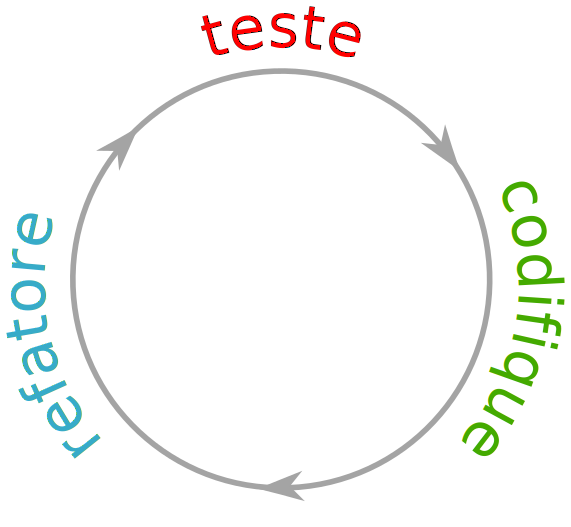
\includegraphics[scale=0.45]{images/ciclo-tdd}
  \label{img:ciclo-tdd}
\end{figure}

\subsection{TDD na prática}
\label{ssub:tdd_na_pratica}

Vejamos agora como isso se dá na prática através de um exemplo retirado do código do kanban-roots.

Precisa-se saber todas as tarefas em uma determinada posição do \textit{kanban} de um projeto. Então, a primeira coisa a ser feita é o teste para o caso mais simples: quando o projeto não tem tarefa alguma naquela determinada posição.

O teste para o caso mais simples pode ser como mostrado no código \ref{code:tdd_spec1}.

% \begin{lstlisting}[caption=Teste para o método Project\#tasks\_by\_position (versão 1),label=code:tdd_spec1]
% # spec/models/project.rb
% describe Project do
%   it "returns all related tasks matching a given position" do
%     project = Factory.create :project
%     project.tasks_by_position(4).should be_empty
%   end
% end
% \end{lstlisting}

\begin{lstlisting}[caption=Teste para o método Project\#tasks\_by\_position (versão 1),label=code:tdd_spec1]
# test/unit/project_test.rb
class ProjectTest < ActiveSupport::TestCase
  def test_tasks_by_position
    project = Factory.create :project
    assert_equal(project.tasks_by_position(4), [])
  end
end
\end{lstlisting}

Ao rodar este teste, ele irá falhar, informando que o método \textit{tasks\_by\_position} sequer existe. Como esta era a falha esperada, escrevemos então o código mais simples para passar neste teste.

\begin{lstlisting}[caption=Código do método Project\#tasks\_by\_position (versão 1),label=code:tdd_code1]
# app/models/project.rb
def tasks_by_position position
  []
end
\end{lstlisting}

Os testes irão passar. Mas a funcionalidade ainda não está completa e, consequentemente, o teste também não.

% \begin{lstlisting}[caption=Teste do método Project\#tasks\_by\_position (versão 2),label=code:tdd_spec2]
% # spec/models/project.rb
% describe Project do
%   it "returns all related tasks matching a given position" do
%     project = Factory.create :project
%     tasks = [Factory.create(:task, :project => project, :position => 1),
%              Factory.create(:task, :project => project, :position => 1)]

%     project.tasks_by_position(4).should be_empty

%     project.should have(2).tasks_by_position(1)
%     project.tasks_by_position(1).should include(*tasks)
%   end
% end
% \end{lstlisting}

\begin{lstlisting}[caption=Teste do método Project\#tasks\_by\_position (versão 2),label=code:tdd_spec2]
# test/unit/project_test.rb
class ProjectTest < ActiveSupport::TestCase
  def test_tasks_by_position
    project = Factory.create :project
    tasks = [Factory.create(:task, :project => project, :position => 1),
             Factory.create(:task, :project => project, :position => 1)]

    assert_equal(project.tasks_by_position(4), [])

    assert_equal(project.tasks_by_position(1).count, 2)
    tasks.each { |task| assert(project.tasks_by_position(1).include?(task)) }
  end
end
\end{lstlisting}

O teste irá falhar, informando que na \hyperref[code:tdd_spec1]{linha 9 do teste} eram esperadas duas tarefas, mas foram obtidas zero. O código então deve ser modificado para passar no novo teste.

\begin{lstlisting}[caption=Código do método Project\#tasks\_by\_position (versão 2),label=code:tdd_code2]
# app/models/project.rb
def tasks_by_position position
  task_list = []
  tasks.each do |task|
    task_list << task if task.position.to_s == position.to_s
  end
  task_list
end
\end{lstlisting}

Desta vez todos os testes os irão passar. Contudo, a cobertura de testes para este método ainda está fraca, o que pode ser resolvido com a adição de mais algumas tarefas em posições diferentes.

% \begin{lstlisting}[caption=Teste do método Project\#tasks\_by\_position (versão 3),label=code:tdd_spec3]
% # spec/models/project.rb
% describe Project do
%   it "returns all related tasks matching a given position" do
%     project = Factory.create :project
%     tasks = [Factory.create(:task, :project => project, :position => 1),
%              Factory.create(:task, :project => project, :position => 1),
%              Factory.create(:task, :project => project, :position => 2),
%              Factory.create(:task, :project => project, :position => 3),
%              Factory.create(:task, :project => project, :position => 3)]

%     project.tasks_by_position(4).should be_empty

%     project.should have(2).tasks_by_position(1)
%     project.tasks_by_position(1).should include(*tasks[0..1])

%     project.tasks_by_position(2).should == [tasks[2]]

%     project.should have(2).tasks_by_position(3)
%     project.tasks_by_position(3).should include(*tasks[3..4])
%   end
% end
% \end{lstlisting}

\begin{lstlisting}[caption=Teste do método Project\#tasks\_by\_position (versão 3),label=code:tdd_spec3]
# test/unit/project_test.rb
class ProjectTest < ActiveSupport::TestCase
  def test_tasks_by_position
    project = Factory.create :project
    tasks = [Factory.create(:task, :project => project, :position => 1),
             Factory.create(:task, :project => project, :position => 1),
             Factory.create(:task, :project => project, :position => 2),
             Factory.create(:task, :project => project, :position => 3),
             Factory.create(:task, :project => project, :position => 3)]

    assert_equal(project.tasks_by_position(4), [])

    assert_equal(project.tasks_by_position(1).count, 2)
    tasks[0..1].each { |task| assert(project.tasks_by_position(1).include?(task)) }

    assert_equal(project.tasks_by_position(2), [tasks[2]])

    assert_equal(project.tasks_by_position(3).count, 2)
    tasks[3..4].each { |task| assert(project.tasks_by_position(3).include?(task)) }
  end
end
\end{lstlisting}

Executando os testes novamente, todos eles passam. Isto indica que já é hora de ir para o item 5 do ciclo TDD e refatorar. Ao comparar o Código \ref{code:tdd_code2} com o Código \ref{code:tdd_code3}, pode-se perceber como o Código \ref{code:tdd_code3} está mais simples e claro e que ao rodar os testes, estes passam mostrando que o comportamento do método não mudou.

\begin{lstlisting}[caption=Código do método Project\#tasks\_by\_position (versão 3),label=code:tdd_code3]
# app/models/project.rb
def tasks_by_position position
  tasks.select { |item| item.position.to_s == position.to_s }
end
\end{lstlisting}

\citeonline{TDDAntiPatterns} descreve vários anti-padrões do TDD e sua leitura é fortemente recomendada.


\section{Behaviour-Driven Development}

Criado em 2006 \cite{IntroducingBDD}, Behaviour-Driven Development (BDD) é uma técnica de desenvolvimento de software cuja amplitude se estende às atividades de design, documentação, validação e verificação, tratando-as de modo unificado \cite{BDDRodrigo}.

Como o nome já diz, Behaviour-Driven Development (Desenvolvimento guiado por comportamento) dá enfase no comportamento ao infez da estrutura. Ao invés de focar em classes e métodos ao escrever os testes, o foco é no comportamento que gera valor para o sistema.

Em TDD, o nome dos testes é baseado na estrutura do código, e isso pode ter um efeito colateral: cria duplicações. Ao escrever testes como o do Código \ref{code:x} nome\_do\_metodo\_de\_teste e o método nome\_do\_metodo é renomeado, o nome do teste também terá que ser renomeado, o que provavelmente é esquecido. Isso torna os testes confusos e desinformativos \cite{ContinuousTesting}.

Por definição, refatorar é melhorar a estrutura e o design do código sem alterar seu comportamento. Nomeando os testes com base no comportamento desejado ao invés da estrutura do código, não apenas torna os testes mais informativos como também torna a refatoração menos custosa.

\textbf{MOSTRAR AQUI O EXEMPLO DO TDD UTILIZANDO BDD}

O BDD é uma evolução do TDD. A grande diferença entre os dois, é que TDD não abrange a validação do software, ou seja, se o software atende os requisitos. Isso muda tudo, pois em BDD, o pensamento não é voltado à verificação, mas sim no comportamento, em \textbf{validar} que o software faz o que deveria fazer, sem deixar também de \textbf{verificar} se está funcionando como deveria.

O Ciclo BDD é engloba o clico TDD visto anteriormente.

BDD vem se tornando um consenso em automação de testes. Contudo, existe controvérsia sobre seu modo de utilização.

Uma das maneiras de escrever testes de aceitação é como texto em língua humana,
ou seja, inglês, português e etc. Nestas ferramentas, os testes são escritos baseados em \textit{steps} (passos), onde os cada step é mapeado para um código real.

No código \ref{code:bdd_cucumber_spec}, é utilizado o cucumber para fazer a especificação de que os comentários devem ser renderizados utilizando a linguagem de marcação Markdown na página de tarefas. Como pode-se ver, o teste é escrito em linguagem que qualquer pessoa, mesmo sem nenhum conhecimento em programação, pode ler e validar. Este é um dos argumentos dos defensores da utilização dessa forma de escrita de testes, que o cliente pode validar os testes, inclusive ele mesmo escrevendo. Existem relatos de que na Globo.com esta abordagem é utilizada (procurar referências) e os clientes escrevem os testes.

\begin{lstlisting}[caption=Especificação ,label=code:bdd_cucumber_spec]
# features/comments.feature
Scenario: Comments should be rendered on tasks page with Markdown syntax
  Given I am a contributor of "sgtran" project
  And I am authenticated
  And I have a task of "sgtran" project
  When I am on the task page
  And I fill in "comment_content" with "# Some content [link](http://exemplo.com)"
  And I press "Comment"
  Then I should see "Some content" in a "h1" tag
  And I should see "link" in an "a" tag
\end{lstlisting}


\begin{lstlisting}[caption=Especificação ,label=code:bdd_spec_1]
# spec/acceptance/comments_spec.rb
feature "Render comments with Markdown syntax" do
  background do
    @owner = Factory.create :contributor
    @project = Factory.create :project
    @task = Factory.create :task, :project => @project, :author => @owner
  end

  scenario "on tasks page" do
    login(@owner.email, @owner.password)
    visit project_task_path(@project, @task)
    fill_in "comment_content", :with => "# Some content [link](http://exemplo.com)"
    click_button "Comment"
    page.should have_xpath("//h1", :text => "Some content")
    page.should have_xpath("//a", :text => "link", :href => "http://exemplo.com")
  end
end
\end{lstlisting}

\section{Integração contínua}

Em uma equipe com vários desenvolvedores, todos trabalhando na elaboração de um mesmo sistema, existe o problema de unificar as diversas alterações feitas na base de código, assegurando que a base continua consistente \cite{ImproveitCI}. Para resolver esse problema, entra em cena a Integração Contínua (IC), que além disso, tem como ponto chave dar um feedback rápido quando a base não está consistente.

\cite{FowlerCI} definiu a IC da seguinte maneira:

\begin{citacao}
Integração Contínua é uma prática de desenvolvimento de software onde os membros de um time integram seu trabalho frequentemente, geralmente cada pessoa integra ao menos uma vez ao dia - podendo haver múltiplas integrações por dia. Cada integração é verificada por um \textit{build} automatizado (incluindo testes) para detectar erros de integração o mais rápido possível. Muitos times acham que essa abordagem leva a uma significante redução nos problemas de integração e permite que um time desenvolva software coeso mais rapidamente.
\end{citacao}

A IC é um dos pilares da agilidade, pois garante que todo o sistema funcione de forma coesa a cada \textit{build}, mesmo que sua equipe seja grande e diversas partes do código estejam sendo alteradas ao mesmo tempo \cite{CaelumCI}.

Existe um debate sobre a periodicidade da integração, que tem relação direta com o tempo de execução da \textit{build}. Para assegurar o rápido feedback, esse tempo de execução deve ser o menor possível, tentando manter sempre menor do que dez minutos \cite{FowlerCI}.

\section{Teste contínuo}
\label{sub:teste_continuo}

Falar aqui de continuous testing.

\section{Dublês de Teste}

Em algumas ocasiões é difícil testar alguns componentes porque eles dependem de outros componentes que não podem ser utilizados em ambiente de teste. Estas situações podem acontecer por esses componentes não estarem disponíveis, por eles não retornam os resultados necessários ou porque executá-los iria trazer efeitos colaterais indesejados. Em outros casos, nossa estratégia de testes requer que nós tenhamos mais controle do comportamento interno do componente.

Quando estamos escrevendo um teste onde não podemos/escolhemos usar componentes reais, podemos substitui-los pelos Dublês de Teste que oferecem uma maneira de isolar as dependências ao criar seus testes, permitindo a utilização de componentes falsos para cumprir os papéis de componentes reais. Com isso, eliminamos complexidade do código dos testes, pois mantemos o código de implementação dos objetos pequeno e com baixo acoplamento.

Os Dublês de Teste não precisam se comportar exatamente como o componente real, eles devem apenas prover a mesma API que o componente real.

\citeonline{XUnit} Define cinco categorias de Dublês de Teste:

\begin{itemize}
\item
Objetos \textbf{\textit{Dummy}} geralmente são utilizados apenas para preencher uma lista de parâmetros e nunca são realmente usados.

\item
Objetos \textbf{\textit{Fake}} são utilizados para substituir funcionalidades reais de um componente por razões diferentes de verificações indiretas de entradas e saídas do componente a ser   testado.

\item
Os \textbf{\textit{Stubs}} provêm respostas prontas para chamadas feitas durante os testes, geralmente não respondendo a qualquer   chamada diferente
das pré-definidas.

\item
Os \textbf{\textit{Spies}} são \textit{Stubs} que também tem gravam algumas informações baseadas em como eles são chamados. Um exemplo   pode ser um serviço de email que grava quantas mensagens foram   enviadas.

\item
\textbf{\textit{Mocks}} são objetos pré-programados para receber determinado conjunto de chamadas, podendo lançar uma exceção se tais chamadas não forem feitas a ele, ou se receber outra chamada diferente das pré-programadas.
\end{itemize}

De modo geral, a utilização de Dublês de Teste é extremamente benéfica para o projeto. Contudo, existem controvérsias, principalmente em relação a utilização do \textit{Mock} \cite{MocksArentStubs}.

%--------------------------------- Bibliografia --------------------------------

\citeoption{abnt-repeated-author-omit=yes}
\bibliographystyle{abnt-alf}
\bibliography{bibliografia}

\end{document}
